
\begin{figure}
  \centering
  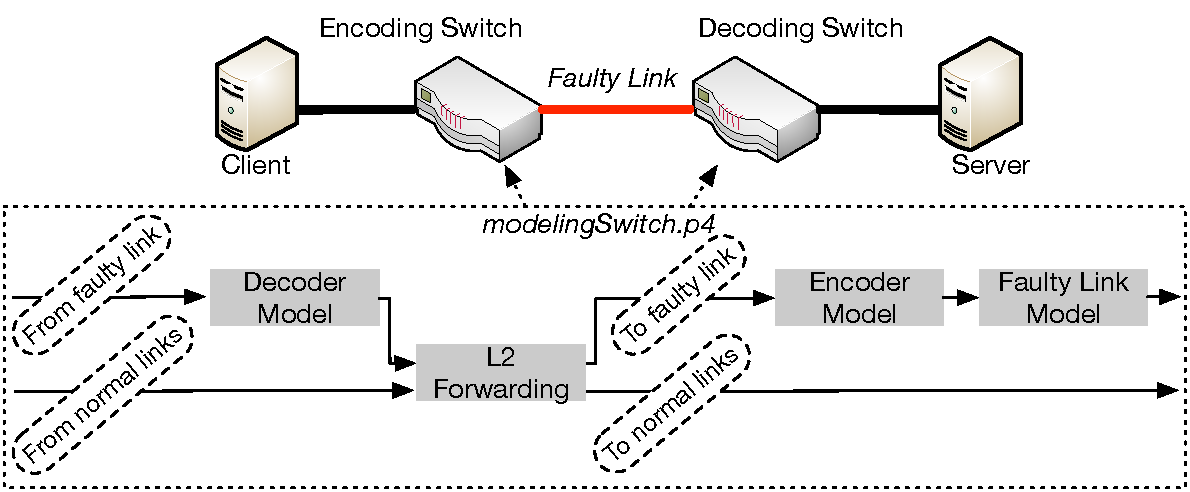
\includegraphics[width=0.4\paperwidth]{figures/lineRateModel.pdf}
  \caption{\label{fig:lineRateModel} P4 pipeline layout for modeling faulty links, encoder, and decoder.}
\end{figure}

To measure the effect of faulty links and
\OurSys at the application level, we implemented a P4 model of lossy links and
the FEC encoder / decoder. The model runs at line  rate alongside the layer 2
forwarding in the Barefoot Tofinos in our  testbed. It captures three
overheads that are important to applications: the bandwidth overhead that the
encoder adds by inserting parity packets and \OurSys headers; the latency
overhead that the decoder adds when recovering lost packets; and the transport
layer overhead that faulty links add by causing packet drops.

\begin{itemize}

\item The \textbf{Encoder Model} encapsulates each packet  egressing on the
faulty link with the \OurSys header and inserts blank  parity packets into the
flow. It tracks per-port block IDs and  packet indices using P4 register
arrays. To generate parity packets, the  model clones the largest packet in
each block with the Tofino's multicast engine. The parity packets are 
delayed until all the data packets in a block egress, using recirculation. 


\item The \textbf{Faulty Link Model} adds a \emph{corruption header} to each packet
egressing the faulty link. The header indicates whether or not the neighbor
switch should consider the packet lost. The model selects packets for corruption
according to a simple binomial distribution implemented with the Tofino's
random number generator.

\item The \textbf{Decoder Model} applies to all packets ingressing from a
modeled faulty link, before any other forwarding logic. For packets that are
not tagged as corrupt, the model simply removes the \OurSys and corruption headers and
allows them to continue to the standard forwarding  pipeline. The model
recirculates corrupt packets until the next block begins, at which point it
decides whether  to recover them based on the number of non-corrupt data and
parity packets it has  observed in the block.  If it counted at least K data
plus parity packets  in the block, the model "recovers" all of the corrupt
packets by removing their corruption headers and forwarding them normally. If
recovery fails, the model simply drops the corrupt packets without forwarding.

\end{itemize}

\begin{figure}
  \centering
  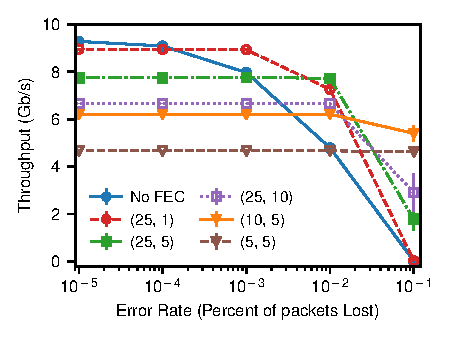
\includegraphics[width=0.3\paperwidth]{figures/lossVsTput.pdf}
  \caption{\label{fig:lossVsTput} Iperf throughput at different loss rates.}
\end{figure}

\begin{figure}
  \centering
  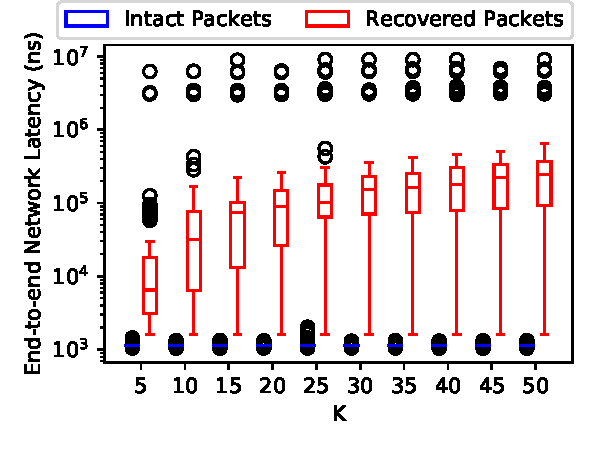
\includegraphics[width=0.3\paperwidth]{figures/udpLatency.pdf}
  \caption{\label{fig:lossVsLatencyUdp} Network latency for a 100 Mb/s UDP flow (H = 5, loss rate = $10 ^{-2}$).}
\end{figure}

\begin{figure}
  \centering
  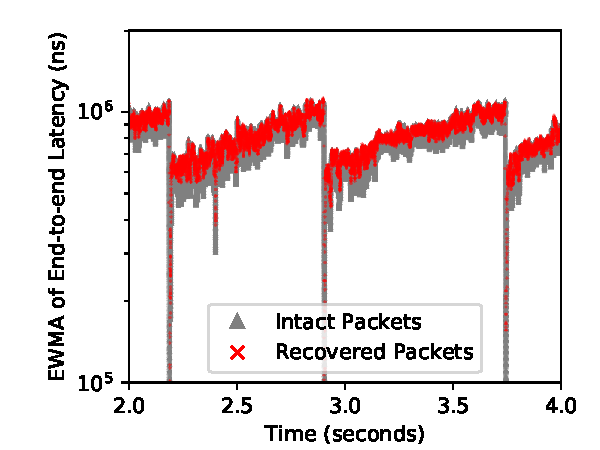
\includegraphics[width=0.3\paperwidth]{figures/tcpLatency.pdf}
  \caption{\label{fig:lossVsLatencyTcp} Network latency for a 9 Gb/s TCP flow (K = 25, H = 5, loss rate = $10 ^{-2}$).}
\end{figure}

Figure~\ref{fig:lossVsTput} shows the benefit that FEC has on TCP throughput
at different rates of packet loss, measured with 60 second iperf trials. With
\OurSys, Iperf sustained  over 5 Gb/s with loss up to $10^{-1}$ (1 out of
every 10 packets dropped). Without \OurSys, Iperf's throughput at that loss
rate was under 25 Mb/s.

% This figure shows the impact of H. 

Figure~\ref{fig:lossVsTput} also shows the bandwidth overhead of  FEC, which
is dominated by the number of parity packets per block ($H$).  At loss rates
greater than or equal to $10^{-4}$ the bandwidth overhead of adding  parity
packets had less of an impact on TCP throughput than lost packets, for  most
configurations tested. To reduce bandwidth overhead, the FEC  can be tuned for the
loss rate of each specific link, which is reportedly stable over
time~\cite{corropt}.


% This figure shows the impact of K.

To understand how FEC impacts latency, we measured the latency  between the
ingress pipeline from the source server and the egress pipeline  to the sink
server, using the nanosecond precision  timestamps of the Tofino, with packets
routed back through the first  switch before egressing to the sink.
Figure~\ref{fig:lossVsLatencyUdp}  plots an EWMA of latency for packets in a
100 Mb/s UDP flow. For  intact packets, latency was low because they did not
invoke  the decoder. For  recovered packets, however, the decoder increased
latency. Average  latency increased with block size because  recovery requires
the decoder to wait until all the parity packets  for a block arrive. The
maximum observed latency for recovered packets  was high, around 9 MS. This
was due to the behavior of the iperf  UDP generator, which periodically paused
for up to 9 MS between  sending packets, to meet the 100 Mb/s target. The high
inter-packet  arrival time stalled the generation of parity packets and thus
the  recovery of any lost packets in the same block.

Figure~\ref{fig:lossVsLatencyTcp} plots a time series of latency EWMA  for TCP
packets in a single maximum rate flow (around 9 Gb/s). The difference in
latency between recovered versus intact packets was almost indistinguishable.
Latency for all packets was not dominated by the decoder, by instead by time
spent  in egress buffers in the switch, which repeatedly filled due to TCPs
congestion  control dynamics, i.e., causing the familiar ``sawtooth'' pattern
in Figure~\ref{fig:lossVsLatencyTcp}. Additionally, the latency for packet
recovery was lower with the TCP workload because average packet rate was
around 1 order of magnitude higher.




